\documentclass[12pt,oneside,final]{thesis}

\usepackage{graphicx}

\usepackage{fancyhdr}    % Use nice looking headers along with the required footer page numbers 



\usepackage[font=singlespacing, labelfont=bf]{caption}
%\usepackage{setspace}
\newlength\TableWidth
\setlength{\paperheight}{11in}
\setlength{\paperwidth}{8.5in}

%Define the header/footer style
\pagestyle{fancy}
\fancyhf{}
\setlength{\headheight}{15pt}
\lhead{\leftmark}
\cfoot{\thepage}
\renewcommand{\headrulewidth}{0pt}
\fancypagestyle{plain}{% Redefine ``plain'' style for chapter boundaries
	\fancyhf{} % clear all header and footer fields
	\fancyfoot[C]{\thepage} % except the center
	\renewcommand{\headrulewidth}{0pt}
	\renewcommand{\footrulewidth}{0pt}}

\begin{document}

\title{ESSAYS ON CONSUMPTION}
\author{Edmund Crawley}
\degreemonth{May}
\degreeyear{2018} 
\dissertation
\doctorphilosophy
\copyrightnotice


% add your chapters, best way is to have separate TeX files for each chapter
%% FRONTMATTER
\begin{frontmatter}

% generate title
\maketitle

\begin{abstract}

Abstract goes here.

\vspace{1cm}

\keywords{Consumption, Marginal Propensity to Consume, Heterogeneity}

\JEL{D12}

\Advisors{\\ Professor Christopher Carroll\\ Professor Jon Faust\\ Professor Jonathan Wright}


\end{abstract}

\begin{acknowledgment}

Thanks!

\end{acknowledgment}

\begin{dedication}
 
This thesis is dedicated to \ldots

\end{dedication}

% generate table of contents
\tableofcontents

% generate list of tables
\listoftables

% generate list of figures
\listoffigures

\end{frontmatter}

\chapter{This is Chapter 1}
\begin{figure}
	\caption{Time Aggregation Induces Serial Correlation}
	\label{fig:TimeAggExample}
	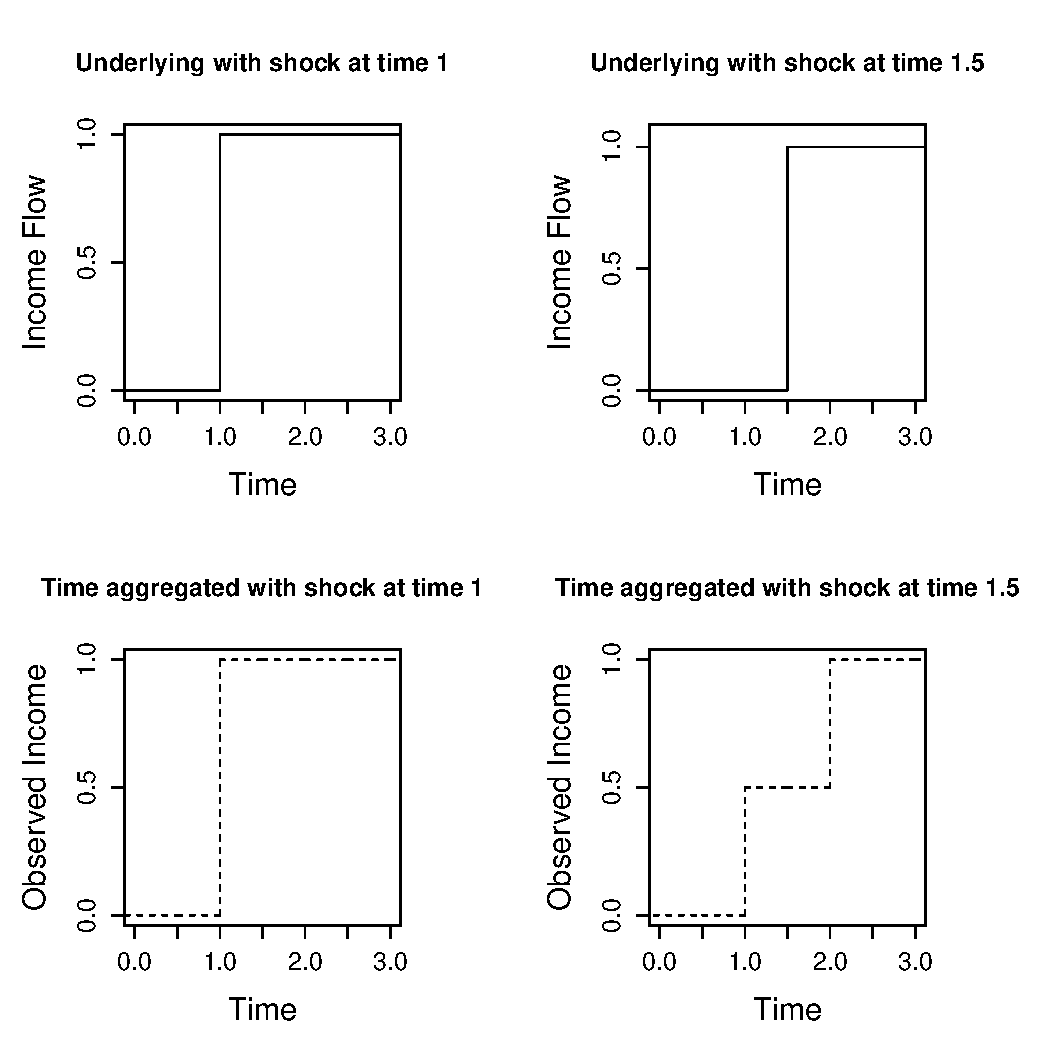
\includegraphics[width=1\textwidth]{TimeAggExample.pdf}
\end{figure}

The first two columns of table \ref{table:Persistence} show that the degree of persistence in the original BPP model makes a big difference to the estimate of $\phi$, while all of the time aggregation models show similar estimates for $\psi$. This suggests the difference we see in the estimates of $\phi$ between BPP original model and the time aggregated model may be driven, at least in part, by misspecification in the model of transitive income shocks. It is reassuring that, in contrast to the BPP model, the values of both $\phi$ and $\psi$ are relatively robust to the exact specification of transitive persistence in the time aggregated model.
The first two columns of table \ref{table:Persistence} show that the degree of persistence in the original BPP model makes a big difference to the estimate of $\phi$, while all of the time aggregation models show similar estimates for $\psi$. This suggests the difference we see in the estimates of $\phi$ between BPP original model and the time aggregated model may be driven, at least in part, by misspecification in the model of transitive income shocks. It is reassuring that, in contrast to the BPP model, the values of both $\phi$ and $\psi$ are relatively robust to the exact specification of transitive persistence in the time aggregated model.
The first two columns of table \ref{table:Persistence} show that the degree of persistence in the original BPP model makes a big difference to the estimate of $\phi$, while all of the time aggregation models show similar estimates for $\psi$. This suggests the difference we see in the estimates of $\phi$ between BPP original model and the time aggregated model may be driven, at least in part, by misspecification in the model of transitive income shocks. It is reassuring that, in contrast to the BPP model, the values of both $\phi$ and $\psi$ are relatively robust to the exact specification of transitive persistence in the time aggregated model.\\
The first two columns of table \ref{table:Persistence} show that the degree of persistence in the original BPP model makes a big difference to the estimate of $\phi$, while all of the time aggregation models show similar estimates for $\psi$. This suggests the difference we see in the estimates of $\phi$ between BPP original model and the time aggregated model may be driven, at least in part, by misspecification in the model of transitive income shocks. It is reassuring that, in contrast to the BPP model, the values of both $\phi$ and $\psi$ are relatively robust to the exact specification of transitive persistence in the time aggregated model.

\input RepTable6.tex

The first two columns of table \ref{table:Persistence} show that the degree of persistence in the original BPP model makes a big difference to the estimate of $\phi$, while all of the time aggregation models show similar estimates for $\psi$. This suggests the difference we see in the estimates of $\phi$ between BPP original model and the time aggregated model may be driven, at least in part, by misspecification in the model of transitive income shocks. It is reassuring that, in contrast to the BPP model, the values of both $\phi$ and $\psi$ are relatively robust to the exact specification of transitive persistence in the time aggregated model.
The first two columns of table \ref{table:Persistence} show that the degree of persistence in the original BPP model makes a big difference to the estimate of $\phi$, while all of the time aggregation models show similar estimates for $\psi$. This suggests the difference we see in the estimates of $\phi$ between BPP original model and the time aggregated model may be driven, at least in part, by misspecification in the model of transitive income shocks. It is reassuring that, in contrast to the BPP model, the values of both $\phi$ and $\psi$ are relatively robust to the exact specification of transitive persistence in the time aggregated model.
The first two columns of table \ref{table:Persistence} show that the degree of persistence in the original BPP model makes a big difference to the estimate of $\phi$, while all of the time aggregation models show similar estimates for $\psi$. This suggests the difference we see in the estimates of $\phi$ between BPP original model and the time aggregated model may be driven, at least in part, by misspecification in the model of transitive income shocks. It is reassuring that, in contrast to the BPP model, the values of both $\phi$ and $\psi$ are relatively robust to the exact specification of transitive persistence in the time aggregated model.
The first two columns of table \ref{table:Persistence} show that the degree of persistence in the original BPP model makes a big difference to the estimate of $\phi$, while all of the time aggregation models show similar estimates for $\psi$. This suggests the difference we see in the estimates of $\phi$ between BPP original model and the time aggregated model may be driven, at least in part, by misspecification in the model of transitive income shocks. It is reassuring that, in contrast to the BPP model, the values of both $\phi$ and $\psi$ are relatively robust to the exact specification of transitive persistence in the time aggregated model.
The first two columns of table \ref{table:Persistence} show that the degree of persistence in the original BPP model makes a big difference to the estimate of $\phi$, while all of the time aggregation models show similar estimates for $\psi$. This suggests the difference we see in the estimates of $\phi$ between BPP original model and the time aggregated model may be driven, at least in part, by misspecification in the model of transitive income shocks. It is reassuring that, in contrast to the BPP model, the values of both $\phi$ and $\psi$ are relatively robust to the exact specification of transitive persistence in the time aggregated model.

%\input C:/Users/edmun/OneDrive/Documents/Research/Dissertation/Chapter1/Tables/RepTable6.tex
%\include{chapter2}
%\include{chapter3}
%\include{appendix}

%% REFERENCES

% if you use BIBTEX
%\bibliographystyle{econometrica}
%\bibliographystyle{IEEEtran}
%\bibliography{Reference_new}


%\begin{vita}
%
%\begin{wrapfigure}{l}{0pt}
%
\includegraphics[width=2in,height=2.5in,clip,keepaspectratio]{rjvheadshot}
%\end{wrapfigure}
%
%\end{vita}
\end{document}
